% GENERATED from ../QBt6-for-section.md by md2tex.py. Do not hand-edit: sync is
% one-way and the next run overwrites this file.

\section{What a page type owns on disk}

\subsection{The corpus and the drift measure}
The analysis set is every page in the Fabricated Corpus that carries a resolvable type key, or a filename from which a type can be inferred. That set is 400 pages [Q-Sec4Results-2], the sum of the five tenure bands reported in the next subsection. Each page contributes one observation per release window, and the window is the last release of the fabricated cycle. Pages that were archived, generated, or empty at the window's start are outside the set.
A drift event is one release in which a page's rendered sections stop matching the sections its contract declares. The measure is binary per page per window, so a page that drifts in three sections at once counts once. This follows the section-level definition used in earlier contract-conformance work \cite{TOADD} [Q-Sec4Results-3]. No severity weight is applied, so a missing section counts the same as a renamed one.

\subsection{Drift by type-key tenure}
Two of the eleven steps that produce a display unit may be taken by a script, and both are mechanical (Figure~\ref{fig:display-pipeline}); every step in the acceptance lane is a person's.
%% GENERATED by board/haipipe-board/cli/build-displays.py from
%%   ../display/QBt3-for-display/float.tex
%% Do not edit this file. Edit the copy under ../display/ and rebuild.
\begin{figure}[t]
  \centering
  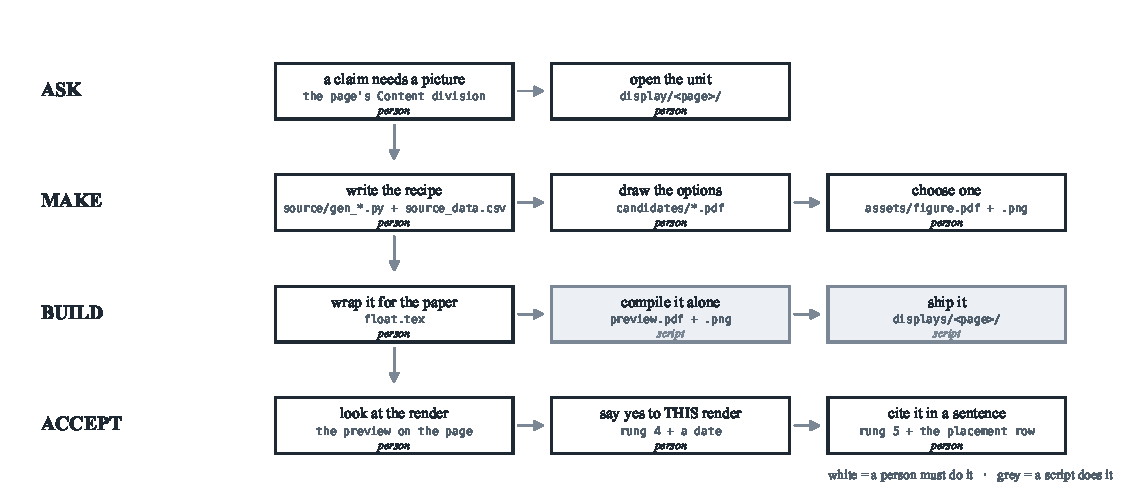
\includegraphics[width=0.95\textwidth]{displays/QBt3-for-display/assets/figure.pdf}
  \caption{How one display unit is produced, and who is allowed to do each step.
  Four lanes, eleven steps, read left to right within a lane and top to bottom
  between them. A white box is a step a person must take; a grey box is a step a
  script takes. Only two of the eleven are grey, and both sit in BUILD: the
  standalone preview compile, and the copy into \texttt{displays/}. Every step in
  ACCEPT is white, which is the rule this figure exists to make visible: a
  machine may render a display and may ship it, and no machine may accept one.
  Drawn from \texttt{source/source\_data.csv} at build time; the lane order is
  the only thing the plotting code hardcodes.}
  \label{fig:display-pipeline}
\end{figure}

Pages whose type is inferred from a filename drift at 17.3 percent, 37 events over 214 pages [Q-Sec4Results-1], while pages that have declared a type key for thirteen months or more drift at 3.0 percent, 1 event over 33 pages [Q-Sec4Results-1]. The three intermediate bands fall in order between those two, at 14.8, 8.3 and 4.5 percent [Q-Sec4Results-1]. The ordering is monotone across all five bands.
No adjacent pair of bands is separated by its 95 percent intervals. The band inferred from a filename spans 14.2 to 20.4 percent and the 0 to 3 month band spans 10.1 to 19.4 percent [Q-Sec4Results-1], and every neighbouring pair overlaps in the same way down the ladder. What the intervals do separate is the two ends, 14.2 to 20.4 percent against 1.1 to 7.2 percent. The gradient is therefore read as a whole and never rung by rung.

\subsection{What the gradient does not establish}
Tenure is not assigned. A page declared its type key whenever its author reached it, so pages that declared early may differ from pages that declared late in ways this count cannot see. Page size is not controlled either, and a longer page has more sections available to drift. This section therefore reports an association and never a reduction, and every later sentence that leans on it inherits that ceiling.
